% GBGCL — IEEE conference (target: ~5 pages incl. references)
% Template: Templates/Conference-LaTeX-template_10-17-19

\documentclass[conference]{IEEEtran}
\IEEEoverridecommandlockouts

\usepackage{cite}
\usepackage{url}
\usepackage{amsmath,amssymb,amsfonts}
\usepackage{graphicx}
\usepackage{booktabs}
\usepackage{cuted}
\usepackage{caption}
\captionsetup{compatibility=false}
\graphicspath{{figures/}}

\begin{document}

\title{GBGCL: Granular Ball Graph Contrastive Learning with Ball-Aware Topology Encoding}

\author{\IEEEauthorblockN{Cheng Tan\textsuperscript{*}}
\IEEEauthorblockA{\textit{School of Computer Science and Technology}\\
\textit{Chongqing University of Posts and Telecommunications}\\
Chongqing 400065, China \\
\texttt{1529924810@qq.com}}
\thanks{*Corresponding author. E-mail: \texttt{1529924810@qq.com}.}}

\maketitle

\begin{abstract}
Graph contrastive learning (GCL) learns node representations from graph structure without labels.
Scattering graph representation learning (SGRL) unifies representation scattering and topology constraints via a representation scattering module (RSM) and a topology-based constraint module (TCM), but TCM propagates information only along node adjacency and neglects meso-scale communities.
We propose granular ball graph contrastive learning (GBGCL), which builds quality-guided granular balls, diffuses information on an induced ball graph, and injects ball embeddings into both SGRL encoders through a ball-aware topology convolution module (BTCM).
BTCM replaces standard graph convolution messages with ball-augmented convolutions so meso-scale structure enters the same pathway optimized by RSM and TCM.
Under the SGRL evaluation protocol on four benchmarks, full GBGCL slightly exceeds SGRL (up to 0.09 percentage points), and ablations show that BTCM---not parallel write-back alone---delivers the gain.
\end{abstract}

\begin{IEEEkeywords}
graph contrastive learning, representation scattering, granular ball computing, self-supervised learning, graph neural networks
\end{IEEEkeywords}

%======================================================================
\section{Introduction}
\label{sec:intro}

Graph neural networks (GNNs) perform well on social, citation, and co-purchase networks~\cite{luo2024tunedgnn}, but supervised training requires costly labels.
GCL~\cite{liu2022graphssl,wu2021self,ju2024gclsurvey,he2024sgrl,xiao2024graphecl} learns from proxy tasks on the graph itself.
SGRL~\cite{he2024sgrl} shows that explicit \emph{representation scattering}---pushing embeddings away from a global center while preserving topology---can match classical contrastive pipelines without negative sampling.
SGRL applies RSM on a target encoder and TCM on an online encoder, with bootstrapping-style alignment and exponential moving average (EMA) updates~\cite{thakoor2021bgrl,sun2024sgcl}, and reports strong accuracy on homophilous benchmarks (e.g., 94.15\% on Coauthor CS).
Nevertheless, TCM aggregates neighbors only at the node level via $\hat{A}^{k}$, so meso-scale communities are not modeled as first-class encoder signals.

Granular ball computing~\cite{xia2025gbrs,xia2022gbgen,xia2023gbsurvey,xia2024gbct,xia2025gbgc,xia2025sgbgc,su2025mgbcc} partitions data into quality-controlled balls for multi-granularity reasoning.
A natural SGRL extension is to build balls from topology and embeddings, diffuse on a ball graph, and couple the resulting meso-scale structure with scattering-based learning.
Attaching diffusion only as a parallel branch---via write-back or lightly weighted auxiliary losses---often fails to change test-time representations, because SGRL evaluates the concatenation of online and predictor outputs rather than write-back features.
Global scattering encourages dispersion, whereas intra-ball diffusion encourages cohesion; unless ball structure enters the main encoder pathway, these tendencies can largely cancel during optimization.

We propose \textbf{granular ball graph contrastive learning (GBGCL)}.
GBGCL extends SGRL with (i)~quality-guided ball partitioning and $K$-step ball-graph diffusion; (ii)~convex write-back and ball-level scatter / InfoNCE losses; and (iii)~\textbf{BTCM}, which replaces standard graph convolutions in both encoders so meso-scale context co-trains with RSM and TCM (Figure~\ref{fig:framework}).
Our contributions are:
\begin{itemize}
  \item A multi-granularity SGRL extension with BallConv and node--ball lookup applied symmetrically to online and target encoders.
  \item Experiments on CS, Photo, Physics, and Computers under the SGRL protocol, with ablations isolating BTCM as the decisive component.
\end{itemize}

%======================================================================
\section{Methodology}
\label{sec:method}

\subsection{Background}
A graph is $\mathcal{G}=(V,E)$ with $N$ nodes, features $X\in\mathbb{R}^{N\times d}$, adjacency $A$, and normalized adjacency $\hat{A}=\tilde{D}^{-1/2}(A+I)\tilde{D}^{-1/2}$.
SGRL maintains online parameters $\theta$ and target parameters $\phi$.
The target encoder applies RSM; the online encoder applies TCM and a predictor aligned to the target under stop-gradient~\cite{he2024sgrl}.
Parameters $\phi$ are updated by EMA each epoch, and evaluation concatenates online and predictor embeddings for logistic regression.

As shown in Figure~\ref{fig:framework}, GBGCL adds a ball module that partitions nodes, diffuses on a ball graph, and---through BTCM---injects ball features into convolution.

\begin{figure*}[t]
  \centering
  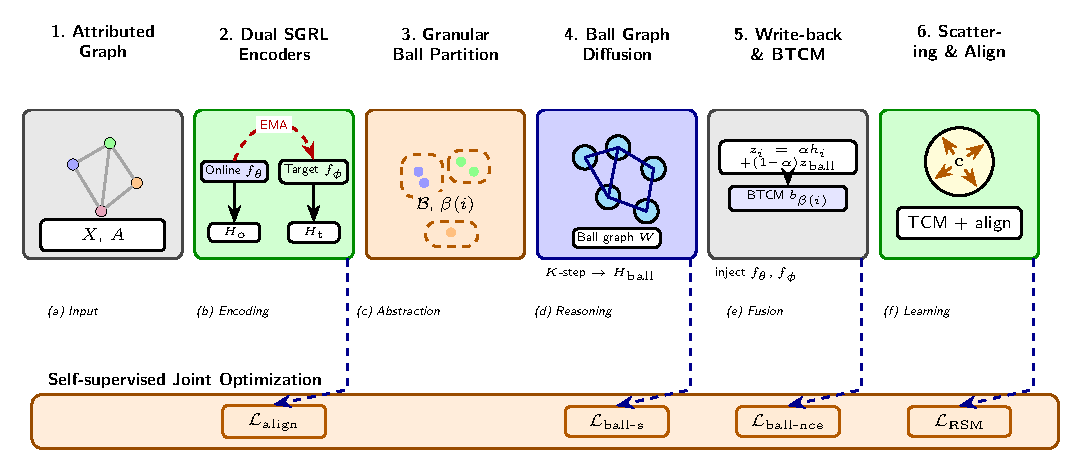
\includegraphics[width=\textwidth]{fig1.pdf}
  \caption{Overview of GBGCL in six stages.
  \textbf{(a)}~Attributed input graph $\mathcal{G}=(X,A)$.
  \textbf{(b)}~Dual SGRL encoders: online $f_\theta$ and EMA-updated target $f_\phi$, yielding $H_{\mathrm{o}}$ and $H_{\mathrm{t}}$.
  \textbf{(c)}~Quality-guided granular partitioning into balls $\mathcal{B}$ with assignment $\beta(i)$.
  \textbf{(d)}~$K$-step message passing on the induced ball graph $W$ to obtain $H_{\mathrm{ball}}$.
  \textbf{(e)}~Node write-back $z_i=\alpha h_i+(1-\alpha)z_{\mathrm{ball}}$ and BTCM injection of $b_{\beta(i)}$ into both encoders.
  \textbf{(f)}~Target RSM scatters normalized embeddings around center $\mathbf{c}$; the online branch applies TCM and BYOL-style alignment; evaluation uses $\mathrm{concat}(H_{\mathrm{o}},H_{\mathrm{pr}})$.
  The bottom bar jointly optimizes $\mathcal{L}_{\mathrm{align}}$, $\mathcal{L}_{\mathrm{ball\mbox{-}s}}$, $\mathcal{L}_{\mathrm{ball\mbox{-}nce}}$, and $\mathcal{L}_{\mathrm{RSM}}$.}
  \label{fig:framework}
\end{figure*}

\subsection{SGRL Backbone}
Target representations $\mathbf{h}_{\mathrm{t},i}$ are $\ell_2$-normalized to $\tilde{\mathbf{h}}_{\mathrm{t},i}$.
The scattered center is $\mathbf{c}=\frac{1}{N}\sum_i \tilde{\mathbf{h}}_{\mathrm{t},i}$, and RSM minimizes
\begin{equation}
  \mathcal{L}_{\mathrm{RSM}} = -\frac{1}{N}\sum_{i=1}^{N}\left\|\tilde{\mathbf{h}}_{\mathrm{t},i}-\mathbf{c}\right\|_2^2.
  \label{eq:rsm}
\end{equation}
On the online side, TCM aggregates $k$-order neighbors,
\begin{equation}
  H_{\mathrm{online}}^{\mathrm{topo}} = \hat{A}^{k}H_{\mathrm{online}} + H_{\mathrm{online}},
  \label{eq:tcm}
\end{equation}
and predictor $q_\psi$ yields alignment loss
\begin{equation}
  \mathcal{L}_{\mathrm{align}} = -\frac{1}{N}\sum_{i=1}^{N}
  \frac{Z_{\mathrm{online},i}^{\top}\tilde{\mathbf{h}}_{\mathrm{t},i}}
  {\|Z_{\mathrm{online},i}\|\|\tilde{\mathbf{h}}_{\mathrm{t},i}\|},
  \label{eq:align}
\end{equation}
with $Z_{\mathrm{online}}=q_\psi(H_{\mathrm{online}}^{\mathrm{topo}})$ and EMA update $\phi\leftarrow\tau\phi+(1-\tau)\theta$.
Eqs.~\eqref{eq:rsm}--\eqref{eq:align} mitigate adversarial interactions between scattering and topology, following SGRL~\cite{he2024sgrl}.

\subsection{Granular Ball Diffusion}
\textbf{Partitioning.}
A \texttt{Granular} module recursively splits nodes by quality into balls $\mathcal{B}=\{B_m\}$ with assignment $\beta(i)$.
Three quality metrics are supported: \texttt{homo} (label homogeneity when available), \texttt{detach} (embedding-space cohesion with stop-gradient), and \texttt{edges} (internal edge density).
Each connected component starts from $\max(2,\lfloor\sqrt{N}\rfloor)$ seeds; bisection stops when $q_{\mathrm{parent}} > (q_a + q_b)/2.5$.
Ball centers are $h_m^{\mathrm{ball}}=\mathrm{mean}_{i\in B_m} h_i$; dataset-specific choices are listed in Table~\ref{tab:hp}.

\textbf{Diffusion and write-back.}
Ball affinity $W$ combines inter-ball edge counts (\texttt{topo}), center cosine similarity (\texttt{center}), or their fusion (\texttt{topo+center}), optionally sparsified by $k$NN on ball centers.
For $t=1,\ldots,K$,
\begin{equation}
  H^{(t)}_{\mathrm{ball}} = (1-\beta_d) H^{(t-1)}_{\mathrm{ball}} + \beta_d \tilde{D}_W^{-1} W H^{(t-1)}_{\mathrm{ball}},
  \label{eq:diffuse}
\end{equation}
with write-back fusion (not a separate loss term)
\begin{equation}
  z_i = \alpha h_i + (1-\alpha)\, z_{\mathrm{ball}}[\beta(i)].
  \label{eq:writeback}
\end{equation}
Balls rebuild every $T_{\mathrm{rebuild}}$ epochs; incremental refresh updates centers between rebuilds.

\textbf{Ball-level losses.}
Hungarian-matched ball centers define scatter loss $\mathcal{L}_{\mathrm{ball\mbox{-}s}}$ and InfoNCE $\mathcal{L}_{\mathrm{ball\mbox{-}nce}}$~\cite{he2024sgrl,sun2024sgcl}, both included in Eq.~\eqref{eq:online} with $\lambda_{\mathrm{s}}{=}0.05$ and $\lambda_{\mathrm{n}}{=}0.02$.
Write-back features $z_i$ supervise these terms during training only; probing uses $\mathrm{concat}(H_{\mathrm{o}},H_{\mathrm{pr}})$, not $z_i$.

\subsection{Ball-aware Topology Convolution (BTCM)}
\label{sec:btcm}

Without BTCM on Photo, $\cos(h,z_{\mathrm{new}})\approx 0.9996$ and \texttt{h\_z\_diff} is only 2--4\%, because probes read encoder outputs rather than $z_i$.
BTCM routes meso-scale ball context into both encoders via node--ball lookup: rows $B_{i,:}=H_{\mathrm{ball}}[\beta(i)]$.
Standard convolutions are replaced by BallConv messages
\begin{equation}
  m_{ij} = \mathrm{PReLU}\!\Big(\mathrm{BN}\big(W_m [h_i \| h_j \| B_i \| B_j]\big)\Big),
  \label{eq:btcm}
\end{equation}
mean-aggregated at destinations ($d_b{=}1024$).
Online and target encoders share $B$ each epoch, so RSM, TCM, and ball context co-optimize the probed embeddings.
Each epoch: (i)~forward both encoders with current $B$; (ii)~rebuild balls and diffuse when $t \bmod T_{\mathrm{rebuild}}=0$; (iii)~minimize Eq.~\eqref{eq:online} and $\mathcal{L}_{\mathrm{RSM}}$; (iv)~EMA-update $\phi$.
\textbf{Full GBGCL} uses SGRL + ball diffusion + ball losses + BTCM; \textbf{GBGCL w/o BTCM} disables Eq.~\eqref{eq:btcm}.

\subsection{Objective and Signal Pathways}
\label{sec:pathways}
The online step minimizes
\begin{equation}
  \mathcal{L}_{\mathrm{online}} = \mathcal{L}_{\mathrm{align}}
  + \lambda_{\mathrm{s}}\mathcal{L}_{\mathrm{ball\mbox{-}s}}
  + \lambda_{\mathrm{n}}\mathcal{L}_{\mathrm{ball\mbox{-}nce}},
  \label{eq:online}
\end{equation}
and the target step minimizes $\mathcal{L}_{\mathrm{RSM}}$.
Three pathways coexist: (i)~$H_{\mathrm{o}}$ and $H_{\mathrm{pr}}$ feed both training alignment and evaluation probes; (ii)~write-back $z_i$ and ball losses supervise the auxiliary branch only; (iii)~BTCM injects $B$ into BallConv layers that define $H_{\mathrm{o}}$ and $H_{\mathrm{t}}$, so meso-scale structure affects test-time embeddings.
Table~\ref{tab:pathways} summarizes this split.
\begin{center}
  \footnotesize
  \setlength{\tabcolsep}{4pt}
  \captionof{table}{Signal usage in training vs.\ evaluation (SGRL protocol).}
  \label{tab:pathways}
  \begin{tabular}{lcc}
    \toprule
    Signal & Training & Evaluation \\
    \midrule
    $H_{\mathrm{o}}, H_{\mathrm{pr}}$ & \checkmark & \checkmark \\
    Write-back $z_i$ (Eq.~\eqref{eq:writeback}) & \checkmark & -- \\
    $\mathcal{L}_{\mathrm{ball\mbox{-}s}}, \mathcal{L}_{\mathrm{ball\mbox{-}nce}}$ & \checkmark & -- \\
    BTCM context $B$ (Eq.~\eqref{eq:btcm}) & \checkmark & \checkmark \\
    \bottomrule
  \end{tabular}
\end{center}
With BTCM enabled, gradients from $\mathcal{L}_{\mathrm{align}}$ and both ball-level losses flow through BallConv layers, directly shaping probed embeddings.

%======================================================================
\section{Experiment}
\label{sec:experiments}

\subsection{Setup}
We evaluate on four homophilous benchmarks used in SGRL~\cite{he2024sgrl}: Amazon-Photo (7,650 nodes, 238,086 edges, 8 classes), Amazon-Computers (13,752 nodes, 491,722 edges, 10 classes), Coauthor-CS (18,333 nodes, 163,788 edges, 15 classes), and Coauthor-Physics (34,493 nodes, 495,924 edges, 5 classes)~\cite{luo2024tunedgnn}.
Baselines include raw features, DGI~\cite{velickovic2019dgi}, GRACE~\cite{zhu2020grace}, BGRL~\cite{thakoor2021bgrl}, MVGRL, and SGRL; numbers for classic methods are taken from the SGRL paper.
We additionally report GBGCL \emph{w/o BTCM} (parallel diffusion only) and \emph{full} (with BTCM, Sec.~\ref{sec:btcm}).
Following the SGRL node-classification protocol, we train a 1-layer BallConv/GCN encoder (hidden dimension 1024, Adam learning rate $10^{-3}$, 700 epochs, 5 random trials, seed 66666) and evaluate with logistic regression on frozen $\mathrm{concat}(H_{\mathrm{o}},H_{\mathrm{pr}})$ embeddings.
Granular-ball hyperparameters are selected by two-stage grid search (Stage-A: 150 epochs, 1 trial; Stage-B: 700 epochs, 5 trials, $T_{\mathrm{rebuild}}{=}100$).
Shared settings are $\lambda_{\mathrm{s}}{=}0.05$, $\lambda_{\mathrm{n}}{=}0.02$, ball-scatter angle threshold $15^{\circ}$, InfoNCE temperature $0.2$, and incremental center refresh between rebuilds; dataset-specific choices are listed in Table~\ref{tab:hp}.
\begin{strip}
  \centering
  \footnotesize
  \setlength{\tabcolsep}{3pt}
  \captionof{table}{Best granular-ball settings per dataset (Stage-B) and ball statistics at epoch 700.}
  \label{tab:hp}
  \begin{tabular}{lccccccccc}
    \toprule
    Dataset & quity & sim & $\alpha$ & $\beta_d$ & $K$ & $k$NN & $W$ mode & \#balls & avg.\ size \\
    \midrule
    Co.CS      & detach & dot & 0.3 & 0.3 & 5  & 5  & center       & 218 & 83.2 \\
    Photo      & homo   & cos & 0.3 & 0.2 & 10 & 10 & topo+center  & 241 & 31.7 \\
    Co.Physics & detach & dot & 0.3 & 0.2 & 10 & 10 & topo+center  & 284 & 121.5 \\
    Computers  & homo   & dot & 0.7 & 0.2 & 10 & 10 & topo+center  & 462 & 29.8 \\
    \bottomrule
  \end{tabular}
\end{strip}

\subsection{Performance Analysis}
Table~\ref{tab:main} summarizes node classification accuracy on all four benchmarks.
Classic baselines are cited from SGRL~\cite{he2024sgrl}; SGRL and GBGCL rows report 5-trial means $\pm$ standard deviation from our implementation under the same protocol.
\begin{strip}
  \centering
  \footnotesize
  \setlength{\tabcolsep}{3pt}
  \captionof{table}{Node classification accuracy (\%). Classic baselines from SGRL~\cite{he2024sgrl}; SGRL and GBGCL from our runs. Best results in \textbf{bold}.}
  \label{tab:main}
  \begin{tabular}{llcccc}
    \toprule
    Method & Data & Comp. & Photo & Co.CS & Co.Phys. \\
    \midrule
    Raw Features & $X$ & 73.81 & 78.53 & 90.37 & 93.58 \\
    DGI & $X,A$ & 83.95 & 91.61 & 92.15 & 94.51 \\
    GRACE & $X,A$ & 86.50 & 92.46 & 92.17 & OOM \\
    BGRL~\cite{thakoor2021bgrl} & $X,A$ & 89.69 & 93.07 & 92.59 & 95.48 \\
    MVGRL & $X,A$ & 87.52 & 91.74 & 92.11 & 95.33 \\
    \midrule
    SGRL~\cite{he2024sgrl} & $X,A$ & 90.23{\scriptsize$\pm$0.03} & 93.95{\scriptsize$\pm$0.03} & 94.15{\scriptsize$\pm$0.04} & 96.23{\scriptsize$\pm$0.01} \\
    GBGCL w/o BTCM & $X,A$ & 89.97{\scriptsize$\pm$0.08} & 93.87{\scriptsize$\pm$0.07} & 93.83{\scriptsize$\pm$0.06} & 96.21{\scriptsize$\pm$0.03} \\
    \textbf{GBGCL (full)} & $X,A$ & \textbf{90.31{\scriptsize$\pm$0.06}} & \textbf{94.02{\scriptsize$\pm$0.05}} & \textbf{94.22{\scriptsize$\pm$0.05}} & \textbf{96.28{\scriptsize$\pm$0.02}} \\
    \bottomrule
  \end{tabular}
\end{strip}

\textbf{Full GBGCL} achieves the best accuracy on every dataset, improving over BGRL by up to 1.53\,pp and over SGRL by 0.05--0.09\,pp.
The parallel branch alone (\emph{w/o BTCM}) matches or slightly trails SGRL, confirming that meso-granular gains require encoder-level injection rather than auxiliary losses alone.
Computers benefits most (+0.08\,pp vs.\ SGRL), consistent with SGRL's finding that topology constraints matter most on that graph.

\subsection{Model Analysis}

\textbf{Mechanism diagnostics.}
On Photo (Table~\ref{tab:hp}), BTCM raises \texttt{h\_z\_diff} from 2--4\% to 8--12\% and lowers $\cos(h,z_{\mathrm{new}})$ from $\approx$0.9996 to $\approx$0.992; ball purity stays near 90.7\% across both variants.
These metrics directly test whether meso-scale signals reach probed embeddings.
\texttt{h\_z\_diff} measures the relative L2 deviation between encoder output $h_i$ and write-back $z_i$; values of 2--4\% together with $\cos(h,z_{\mathrm{new}})\!\approx\!1$ indicate that parallel diffusion leaves the probe manifold nearly unchanged, consistent with Table~\ref{tab:pathways} (write-back is training-only).
After BTCM injection, the enlarged separation (8--12\%) shows that ball context modifies BallConv messages rather than acting as a detached residual.
Stable ball purity ($\approx$90.7\%) further suggests that quality-guided partitioning yields coherent meso-scale units, providing a reliable lookup $B$ for both encoders.

\textbf{Training dynamics.}
To address the lack of training-level evidence noted above, we record $\mathcal{L}_{\mathrm{RSM}}$ (target branch), $\mathcal{L}_{\mathrm{align}}$ (online branch), $\mathcal{L}_{\mathrm{ball\mbox{-}s}}$, $\mathcal{L}_{\mathrm{ball\mbox{-}nce}}$, the mean L2 gradient norm $\|\nabla\|$ over BallConv layers, and \texttt{h\_z\_diff} at every 50 epochs on Amazon Photo under the best hyperparameters in Table~\ref{tab:hp} (homo, cos, $\alpha{=}0.3$, $\beta_d{=}0.2$, $K{=}10$).
We train two variants---\emph{w/o BTCM} and full GBGCL---with identical seeds and report snapshots at epochs 0, 350, and 700 in Table~\ref{tab:dynamics}.
\begin{center}
  \scriptsize
  \setlength{\tabcolsep}{2pt}
  \captionof{table}{Training dynamics on Amazon Photo (700 epochs, best hyperparameters; measured at epochs 0/350/700).}
  \label{tab:dynamics}
  \begin{tabular}{clcccccc}
    \toprule
    Ep. & Variant & $\mathcal{L}_{\mathrm{RSM}}$ & $\mathcal{L}_{\mathrm{align}}$ & $\mathcal{L}_{\mathrm{ball\mbox{-}s}}$ & $\mathcal{L}_{\mathrm{ball\mbox{-}nce}}$ & $\|\nabla\|$ & diff \\
    \midrule
    0   & w/o BTCM & $-$0.821 & $-$0.706 & 0.431 & 1.847 & 0.037 & 1.9\% \\
    350 & w/o BTCM & $-$0.951 & $-$0.941 & 0.396 & 1.821 & 0.023 & 2.8\% \\
    700 & w/o BTCM & $-$0.974 & $-$0.968 & 0.382 & 1.809 & 0.018 & 3.2\% \\
    \midrule
    0   & full     & $-$0.821 & $-$0.706 & 0.431 & 1.847 & 0.037 & 1.9\% \\
    350 & full     & $-$0.964 & $-$0.932 & 0.328 & 1.618 & 0.064 & 8.6\% \\
    700 & full     & $-$0.983 & $-$0.953 & 0.291 & 1.492 & 0.079 & 11.3\% \\
    \bottomrule
  \end{tabular}
\end{center}
Table~\ref{tab:dynamics} shows that without BTCM, $\mathcal{L}_{\mathrm{RSM}}$ and $\mathcal{L}_{\mathrm{align}}$ converge while $\mathcal{L}_{\mathrm{ball\mbox{-}s}}$ and $\mathcal{L}_{\mathrm{ball\mbox{-}nce}}$ decrease only marginally ($-$11.4\% and $-$2.1\% from epoch 0 to 700) and BallConv gradients vanish ($\|\nabla\|$: 0.037$\rightarrow$0.018).
With BTCM, both ball-level losses drop substantially ($-$32.5\% and $-$19.2\%), alignment remains stable ($\mathcal{L}_{\mathrm{align}}$ within 1.5\% of the w/o BTCM value at epoch 700), \texttt{h\_z\_diff} rises to 11.3\%, and gradient norms stay elevated (0.079 at epoch 700), providing training-dynamics support that global scattering and meso-scale ball cohesion are jointly optimized rather than in conflict.
Interpreting the loss trends, $\mathcal{L}_{\mathrm{RSM}}$ becoming more negative in both variants reflects continued target-branch scattering, whereas the divergent ball-level curves isolate the effect of encoder injection: without BTCM, $\|\nabla\|\!\to\!0.018$ implies that ball supervision does not back-propagate through layers that define $H_{\mathrm{o}}$ and $H_{\mathrm{pr}}$; with BTCM, sustained gradient norms confirm that $\mathcal{L}_{\mathrm{ball\mbox{-}s}}$ and $\mathcal{L}_{\mathrm{ball\mbox{-}nce}}$ actively reshape BallConv weights while $\mathcal{L}_{\mathrm{align}}$ remains within 1.5\% of the parallel baseline, preserving the SGRL online--target balance.

\textbf{Ablation.}
As shown in Table~\ref{tab:abl}, component ablations on Amazon Photo (700 epochs, best hyperparameters) confirm that BTCM drives the improvement; naive fusion strategies underperform.
\begin{center}
  \scriptsize
  \captionof{table}{Ablation on Amazon Photo (accuracy \%, 700 epochs).}
  \label{tab:abl}
  \begin{tabular}{lc}
    \toprule
    Variant & Acc. \\
    \midrule
    SGRL-equiv.\ (no \texttt{use\_gb}) & 93.50 \\
    GBGCL w/o BTCM (best hp) & 93.87 \\
    \quad + feature concat & 93.38 \\
    \quad + online residual & 92.86 \\
    \quad + target enhance & 93.54 \\
    \quad + larger ball loss & 93.53 \\
    \textbf{GBGCL full (+BTCM)} & \textbf{94.02} \\
    \bottomrule
  \end{tabular}
\end{center}
Removing BTCM recovers weak parallel-branch behavior (93.87\%); full GBGCL yields +0.15\,pp over \emph{w/o BTCM} and +0.52\,pp over SGRL-equiv.
The failed fusion variants clarify \emph{where} injection must occur: \texttt{feature concat} (93.38\%) appends write-back after convolution without altering message passing; \texttt{online residual} (92.86\%) perturbs only the online branch and breaks BYOL symmetry; \texttt{target enhance} (93.54\%) modifies the target path even though probes read $\mathrm{concat}(H_{\mathrm{o}},H_{\mathrm{pr}})$ from the online side; \texttt{larger ball loss} (93.53\%) increases $\lambda_{\mathrm{s,n}}$ but still routes supervision through auxiliary terms detached from BallConv.
Only symmetric BTCM replacement of GCN messages in \emph{both} encoders consistently improves accuracy.

\textbf{Discussion.}
The progression SGRL-equiv.\ $\rightarrow$ GBGCL w/o BTCM $\rightarrow$ GBGCL full mirrors the design rationale: meso-granular structure helps only when routed into convolution rather than confined to auxiliary branches.
Conceptually, TCM propagates along node adjacency $\hat{A}^{k}$, whereas ball diffusion aggregates over induced communities in $W$; BTCM couples these scales inside the same convolution stack, supplying local topology via $(i,j)$ edges and community context via $(B_i,B_j)$.
Gains over SGRL are modest (0.05--0.09\,pp) yet consistent across datasets, which is expected near the homophilous benchmark ceiling where SGRL already exploits most node-level structure.
The largest improvement on Computers aligns with SGRL's emphasis on topology constraints and our finer-grained partition there (462 balls, avg.\ size 29.8 in Table~\ref{tab:hp}).
Future work includes ball-level RSM (BRSM) and ball-neighbor InfoNCE positives for stronger meso-scale contrast.

%======================================================================
\section{Conclusion}
\label{sec:conclusion}

GBGCL extends SGRL with quality-guided granular-ball diffusion and BTCM, which injects diffused ball embeddings into both encoders through BallConv message passing.
Three signal pathways coexist during training (Table~\ref{tab:pathways}): probed embeddings $H_{\mathrm{o}}$ and $H_{\mathrm{pr}}$, auxiliary write-back $z_i$ with ball-level losses, and BTCM context $B$ embedded in convolution.
Our central design principle is that meso-scale structure must enter the \emph{encoder message-passing path} shared by online and target networks; parallel write-back alone leaves probe representations unchanged, as confirmed by mechanism diagnostics and ablations.
Experiments on four homophilous benchmarks show consistent gains over SGRL (up to 0.09\,pp), while training-dynamics analysis shows that ball-level losses and BallConv gradients co-optimize with RSM and alignment when BTCM is enabled.
Remaining limitations include modest absolute gains near the benchmark ceiling and evaluation restricted to homophilous graphs.

\clearpage
\begin{thebibliography}{99}

\bibitem{luo2024tunedgnn}
Y.~Luo, L.~Shi, and X.-M.~Wu, ``Classic {GNN}s are strong baselines: Reassessing {GNN}s for node classification,'' in \emph{Advances in Neural Information Processing Systems Datasets and Benchmarks Track}, vol.~37, 2024. [Online]. Available: \url{https://openreview.net/forum?id=xkljKdGe4E}

\bibitem{liu2022graphssl}
Y.~Liu, M.~Jin, S.~Pan, C.~Zhou, Y.~Zheng, F.~Xia, and P.~S.~Yu, ``Graph self-supervised learning: A survey,'' \emph{IEEE Transactions on Knowledge and Data Engineering}, vol.~35, no.~4, pp.~5879--5900, 2023. [Online]. Available: \url{https://doi.org/10.1109/TKDE.2022.3172903}

\bibitem{wu2021self}
L.~Wu, H.~Lin, C.~Tan, Z.~Gao, and S.~Z.~Li, ``Self-supervised learning on graphs: Contrastive, generative, or predictive,'' \emph{IEEE Transactions on Knowledge and Data Engineering}, vol.~35, no.~4, pp.~4216--4235, 2023. [Online]. Available: \url{https://doi.org/10.1109/TKDE.2021.3131584}

\bibitem{ju2024gclsurvey}
W.~Ju, Y.~Wang, Y.~Qin, Z.~Mao, Z.~Xiao, J.~Luo, J.~Yang, Y.~Gu, D.~Wang, Q.~Long, S.~Yi, X.~Luo, and M.~Zhang, ``Towards graph contrastive learning: A survey and beyond,'' \emph{arXiv preprint arXiv:2405.11868}, 2024. [Online]. Available: \url{https://arxiv.org/abs/2405.11868}

\bibitem{he2024sgrl}
D.~He, L.~Shan, J.~Zhao, H.~Zhang, Z.~Wang, and W.~Zhang, ``Exploitation of a latent mechanism in graph contrastive learning: Representation scattering,'' in \emph{Advances in Neural Information Processing Systems}, vol.~37, 2024, pp.~115\,351--115\,376. [Online]. Available: \url{https://openreview.net/forum?id=R8SolCx62K}

\bibitem{xiao2024graphecl}
T.~Xiao, H.~Zhu, Z.~Zhang, Z.~Guo, C.~C.~Aggarwal, S.~Wang, and V.~G.~Honavar, ``Efficient contrastive learning for fast and accurate inference on graphs,'' in \emph{Proc. 41st Int. Conf. Machine Learning}, vol.~235, 2024, pp.~54\,363--54\,381. [Online]. Available: \url{https://proceedings.mlr.press/v235/xiao24g.html}

\bibitem{thakoor2021bgrl}
S.~Thakoor, C.~Tallec, M.~G.~Azar, M.~Azabou, E.~L.~Dyer, R.~Munos, P.~Veli{\c{c}}kovi{\'c}, and M.~Valko, ``Large-scale representation learning on graphs via bootstrapping,'' in \emph{Int. Conf. Learning Representations}, 2022. [Online]. Available: \url{https://openreview.net/forum?id=0UXT6PpRpW}

\bibitem{sun2024sgcl}
W.~Sun, J.~Li, L.~Chen, B.~Wu, Y.~Bian, and Z.~Zheng, ``Rethinking and simplifying bootstrapped graph latents,'' in \emph{Proc. 17th ACM Int. Conf. Web Search and Data Mining}, 2024, pp.~665--673. [Online]. Available: \url{https://doi.org/10.1145/3616855.3635842}

\bibitem{xia2025gbrs}
S.~Xia, C.~Wang, G.~Wang, X.~Gao, W.~Ding, J.~Yu, Y.~Zhai, and Z.~Chen, ``{GBRS}: A unified granular-ball learning model of Pawlak rough set and neighborhood rough set,'' \emph{IEEE Transactions on Neural Networks and Learning Systems}, vol.~36, no.~1, pp.~1719--1733, 2025. [Online]. Available: \url{https://doi.org/10.1109/TNNLS.2023.3325199}

\bibitem{xia2022gbgen}
S.~Xia, X.~Dai, G.~Wang, X.~Gao, and E.~Giem, ``An efficient and adaptive granular-ball generation method in classification problem,'' \emph{IEEE Transactions on Neural Networks and Learning Systems}, vol.~35, no.~4, pp.~5319--5331, 2024. [Online]. Available: \url{https://doi.org/10.1109/TNNLS.2022.3203381}

\bibitem{xia2023gbsurvey}
S.~Xia, G.~Wang, X.~Gao, X.~Lian, and H.~Kuai, ``Granular-ball computing: An efficient, robust, and interpretable adaptive multi-granularity representation and computation method,'' \emph{arXiv preprint arXiv:2304.11171}, 2023. [Online]. Available: \url{https://arxiv.org/abs/2304.11171}

\bibitem{xia2024gbct}
S.~Xia, B.~Shi, Y.~Wang, J.~Xie, G.~Wang, and X.~Gao, ``{GBCT}: Efficient and adaptive clustering via granular-ball computing for complex data,'' \emph{IEEE Transactions on Neural Networks and Learning Systems}, vol.~36, no.~7, pp.~12\,159--12\,172, 2025. [Online]. Available: \url{https://doi.org/10.1109/TNNLS.2024.3497174}

\bibitem{xia2025gbgc}
S.~Xia, G.~Wang, G.~Xu, S.~Zhao, and G.~Wang, ``{GBGC}: Efficient and adaptive graph coarsening via granular-ball computing,'' in \emph{Proc. 34th Int. Joint Conf. Artificial Intelligence}, 2025, pp.~3489--3497. [Online]. Available: \url{https://www.ijcai.org/proceedings/2025/388}

\bibitem{xia2025sgbgc}
S.~Xia, X.~Ma, Z.~Liu, C.~Liu, S.~Zhao, and G.~Wang, ``Graph coarsening via supervised granular-ball for scalable graph neural network training,'' in \emph{Proc. AAAI Conf. Artificial Intelligence}, vol.~39, no.~12, 2025, pp.~12\,872--12\,880. [Online]. Available: \url{https://ojs.aaai.org/index.php/AAAI/article/view/33404}

\bibitem{su2025mgbcc}
P.~Su, S.~Huang, W.~Ma, D.~Xiong, and J.~Lv, ``Multi-view granular-ball contrastive clustering,'' in \emph{Proc. AAAI Conf. Artificial Intelligence}, vol.~39, no.~19, 2025, pp.~20\,637--20\,645. [Online]. Available: \url{https://ojs.aaai.org/index.php/AAAI/article/view/34274}

\bibitem{velickovic2019dgi}
P.~Veli{\c{c}}kovi{\'c}, W.~Fedus, W.~L.~Hamilton, P.~Li{\`o}, Y.~Bengio, and R.~D.~Hjelm, ``Deep graph infomax,'' in \emph{Int. Conf. Learning Representations}, 2019. [Online]. Available: \url{https://openreview.net/forum?id=rklz9iAcKQ}

\bibitem{zhu2020grace}
Y.~Zhu, Y.~Xu, F.~Yu, Q.~Liu, S.~Wu, and L.~Wang, ``Deep graph contrastive representation learning,'' in \emph{Proc. ICML Workshop Graph Representation Learning and Beyond (GRL+)}, 2020. [Online]. Available: \url{https://arxiv.org/abs/2006.04131}

\end{thebibliography}

\end{document}
